43. $\cfrac{(x-3)^2(x^2-3x-10)}{x^2+8x+16}\leqslant0\Leftrightarrow\cfrac{(x-3)^2(x-5)(x+2)}{(x+4)^2}\leqslant0.$ Применив метод интервалов, найдём ответ: $x\in[-2;5].$
\begin{figure}[ht!]
\center{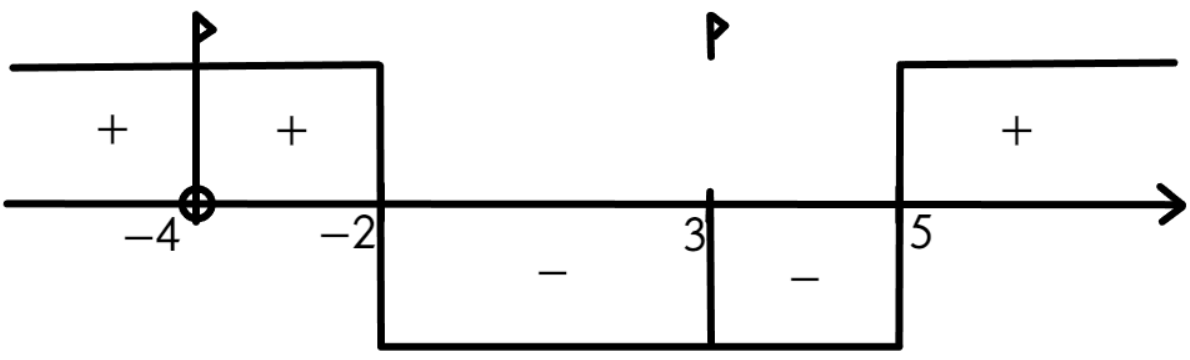
\includegraphics[scale=0.35]{ner9-43.png}}
\end{figure}\\
